\chapter{The Art of Combinatorial Thinking}
\section{Binomial Coefficients}
This section aims to push forward our familiarity with binomial coefficients which we have gained from the previous chapter. We do so by outlining proofs of a few standard combinatorial identities.
\begin{comment}
Three numbers out of the $n+1$ choices say $a_{1}<a_{2}<a_{3}$. Now argue for the first three sums based on which one of these is chosen first. 

The first sum corresponds to choosing $a_2$. The second sum corresponds to choosing  $a_{3}$. The third sum corresponds to choosing $a_{1}$.

\begin{question}
	For all $n\geq r\geq 0$ we have 
	 \[
		 \binom{r}{r}+\binom{r+1}{r}+\cdots+\binom{n}{r} = \binom{n+1}{r+1}
	.\] 
\end{question}
Give a proof using lattice paths. 
RHS is the number of lattice paths from $(0,0)\to (r+1,n-r)$. For the LHS what happens before the last E step.

The idea is not always to prove equalities. In fact more often than not we will be interested in proving inequalities
 \begin{question}
	 \binom{2n}{n}<4^n
\end{question}
Convert binary to lattice: 0 to N, 1 to E and so on.

\begin{question}
	For all $n>0$. \[
		\sum_{k=0}^{n} 2^k\binom{n}{k} = 3^n
	\]
\end{question}

\begin{question}
	For $n>0$  \[
		2\binom{2n-1}{n} = \binom{2n}{n}
	.\] 
\end{question}
Give two proofs. One using Pascal's identity. The other by choosing sets.
\end{comment}

\begin{claim}
\[
\sum_{k=1}^{n}k\binom{n}{k}^2 = n\binom{2n-1}{n-1}
\]
\end{claim}
\begin{proof}
Let $J$ be a collection of $2n$ objects which is partitioned into $2$ equal sub-collections $J_1$ and $J_2$. Now, we want to make a choice of $n$ elements from $J$ which includes a distinguished element, say $x$ from $J_1$ (or equivalently $J_2$). Since there are $n$ ways to choose the said distinguished element, and $\binom{2n-1}{n-1}$ ways to choose the rest of the $n-1$ elements, in all we have \[
n\binom{2n-1}{n-1}
\] ways to make the said choice. Alternatively, we can also choose $k$ elements from $J_1$ in $\binom{n}{k}$ ways, $n-k$ elements from $J_2$ in $\binom{n}{n-k}$ ways, and then choose the distinguished element from $J_1$ (or equivalently $J_2$) in $1\leq k\leq n$ ways. Thus far, we have proved
\[
\sum_{k=1}^{n}k\binom{n}{k}\binom{n}{n-k} = n\binom{2n-1}{n-1}.
\]
Since by \cref{r:1.2} \[
\binom{n}{k} = \binom{n}{n-k},
\]
we are done. 
\end{proof}
\begin{claim}
\[
\sum_{k=1}^{n}k\binom{n}{k} = n2^{n-1}
\]
\end{claim}
\begin{proof}
In a class of $n$ students, a football coach wants to choose students to form a football team of $1\leq k\leq n$ players. Additionally, the coach also wants one of $k$ students to be the captain of the team. Since the representative can be chosen in $n$ ways and the remaining set of students can be chosen in $2^{n-1}$ ways, the team can be chosen in $n2^{n-1}$ ways.  Alternatively, the coach can select $k$ players out of $n$ in $\binom{n}{k}$ ways, and then choose the captain in $k$ ways. Since $0<k\leq n$, we are done. 
\end{proof}

\begin{claim}
\[
\sum_{i=1}^{n}i(n-1) = \sum_{i=1}^{n}\binom{i}{2} = \sum_{i=0}^{n-2}\binom{n-i}{2} = \binom{n+1}{3} 
\]
\end{claim}
\begin{proof}
It is clear that $\binom{n+1}{3}$ is the number of ways to choose $3$ numbers, say $a_{1}<a_{2}<a_{3}$, from the $n+1$-element set $\{a_1,\cdots,a_{n+1}\}$. Now we argue based on which one of these three is chosen first. If 
\end{proof}
\begin{claim}
For all $n\geq r\geq 0$ we have 
\[
\binom{r}{r}+\binom{r+1}{r}+\cdots+\binom{n}{r} = \binom{n+1}{r+1}
.\] 
\end{claim}
\begin{proof}
We give a double-counting argument. Noitce how $\binom{n+1}{r+1}$ counts the number of ways to choose $(r+1)$-element subsets of $[n+1]=\{1,\ldots,n+1\}$. A choice of the said subsets can also be made by first fixing the largest of the $r+1$ numbers. This is given by $\binom{r}{r}+\cdots+\binom{n}{r}$. 
\end{proof}
\begin{claim}
$\binom{2n}{n}<4^n$
\end{claim}
\begin{proof}
The claim follows from the simple observation that \[
4^{n} = (1+1)^{2n} = \sum_{i=0}^{2n} \binom{2n}{i} = \binom{2n}{n}+\underbrace{\sum_{0\leq i\leq 2n, i\neq n} \binom{2n}{i}}_{>0}. 
\]
\end{proof}
\begin{claim}[Chu-Vandermonde Identity]
\[\binom{2n}{n} = \sum_{k=0}^{n} \binom{n}{k}^2\]
\end{claim}
\begin{proof}
Once again, by \cref{r:1.2}, notice how \[
\sum_{k=1}^n\binom{n}{k}^2 = \sum_{k=1}^{n}\binom{n}{k}\binom{n}{n-k}.
\] Now we argue combinatorially. Let $J$ be a collection of $2n$ objects which is partitioned into $2$ equal sub-collections $J_1$ and $J_2$. Any choice of $n$ elements from $J$ involves choosing $k$ elements from $J_1$ and $n-k$ elements from $J_2$ where $0\leq k\leq n$. 
\end{proof}
\begin{claim}
	For all $n>0$. \[
		\sum_{k=0}^{n} 2^k\binom{n}{k} = 3^n
	\]
\end{claim}
\begin{proof}
We give a double-counting argument. Notice how $3^n$ is the number of $n$-bit ternary strings. Each such string will have $n-k$-many $0$s in it where $0\leq k \leq n$. Such a string can be chosen in $\binom{n}{n-k}=\binom{n}{k}$ ways, and the remaining $k$ bits (which can now only either be $1$s or $2$s) can be chosen in $2^k$ ways. This completes the proof. 
\end{proof}
\section{Catalan Numbers}
This section introduces a set of problems that are seemingly distinct but share a common underlying sequence of numbers called the Catalan numbers. We shall show this commonality by setting up appropriate bijections between the said problems. 
\begin{question}
Recall how with \cref{q:1.8} we counted the number of lattice paths from $(0,0)$ to $(m,n)$. Count the number of lattice paths, $a_1(n)$, from $(0,0)$ to $(n,n)$ which never go below the $x=y$ diagonal.
\end{question}
\begin{figure}[H]
    \centering
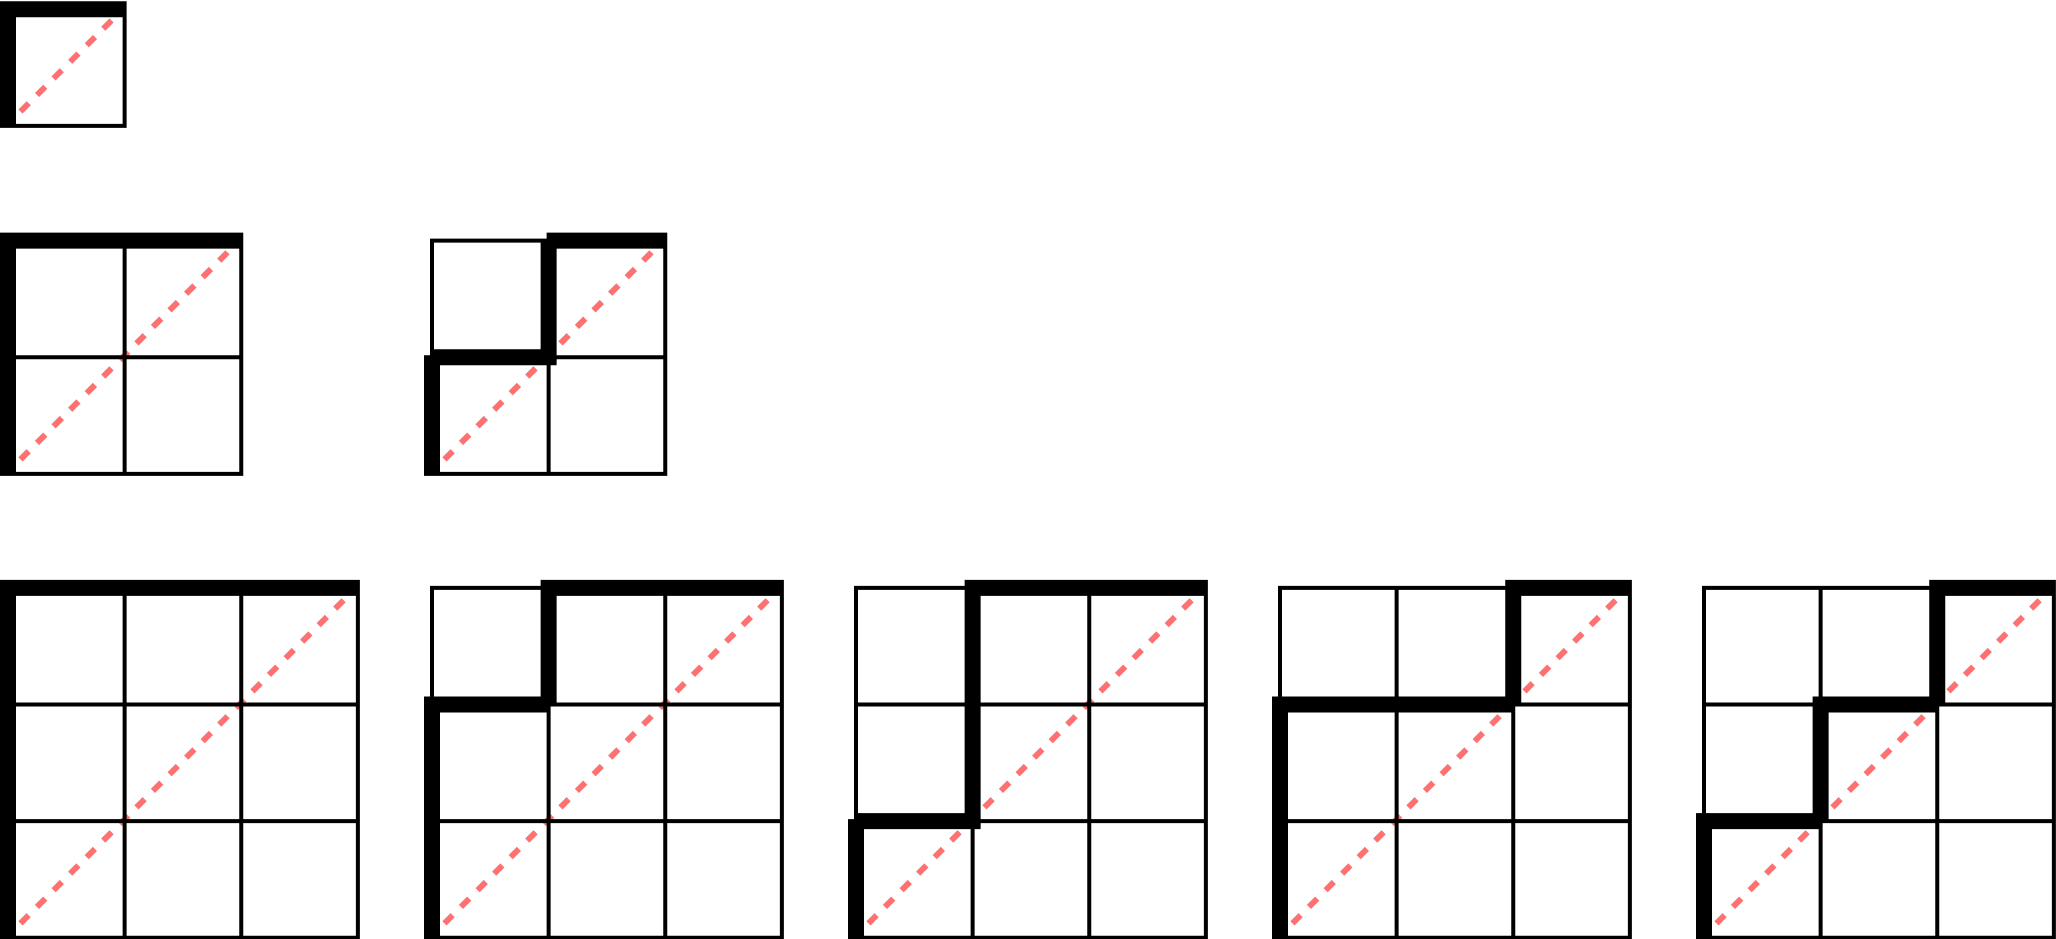
\includegraphics[width=0.8\linewidth]{Images/Figure11.png}
    \caption{All possible lattice paths which don't go below the diagonal for cases $n=1,2,3$}
    \label{f:3.21}
\end{figure}    
\begin{remark}
Notice that reflecting each path in \cref{f:3.21} across the main diagonal produces a lattice path that remains strictly below it. This bijection clearly shows that $a_1(n)$, the number of lattice paths that do not fall below the diagonal is the same as $a_2(n)$, the number of those that do not rise above it.
\end{remark}
\begin{question}
Count the number of ways $a_3(n)$, of filling a $2\times n$ grid with elements from the set $\{0,1,2,3,\cdots,2n\}$ such that all elements are unique, increasing row-wise, and decreasing column-wise.
\end{question}
\begin{solution}
\begin{figure}[H]
    \centering
    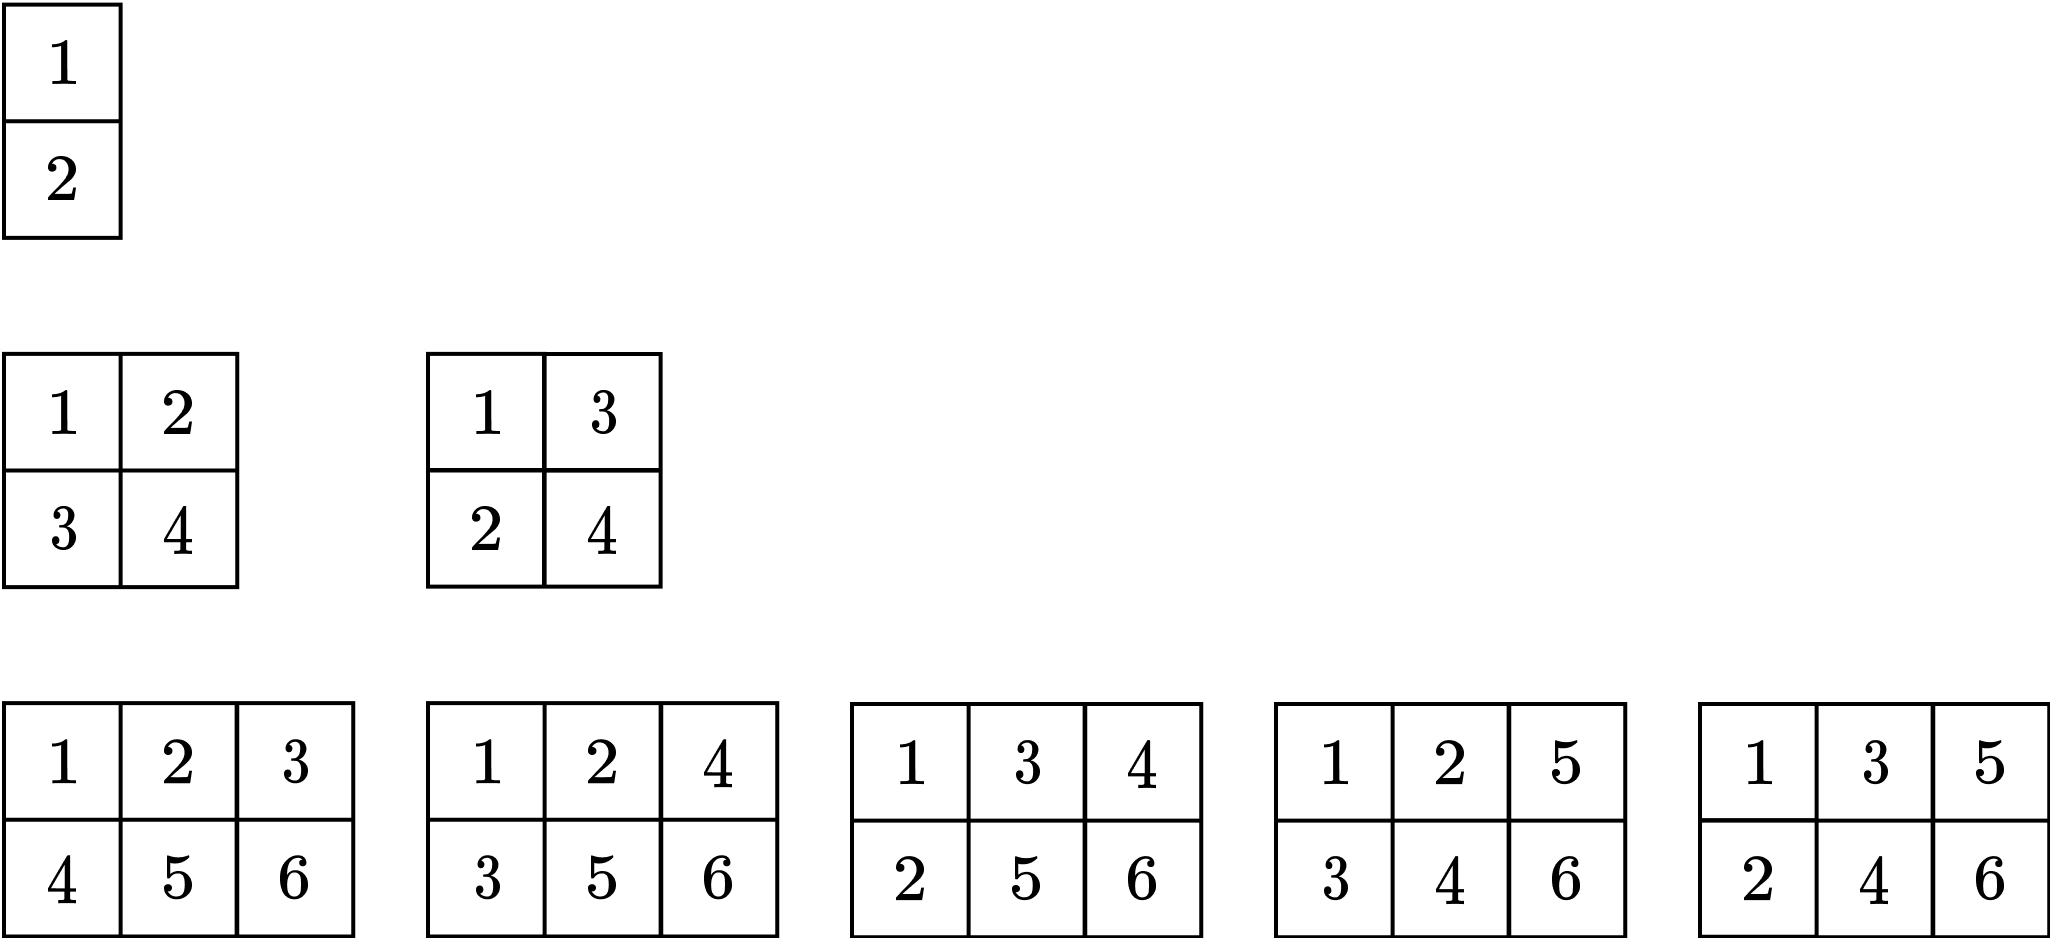
\includegraphics[width=0.8\linewidth]{Images/Figure12.png}
    \caption{All possible such arrangements of order $2\times n$ for cases $n=1,2,3$}
    \label{f:3.22}
\end{figure}
A bijection presents itself when \cref{f:3.21} and \cref{f:3.22} are compared. Namely, the entries in the first row of the $2\times n$ grid correspond to when an $N$-step in our lattice path occurs, and the entries in the second row correspond to when an $E$-step in our lattice path occurs.     
\end{solution}
\begin{question}
Count the number of Dyck paths $a_4(n)$, from $(0,0)$ to $(2n,0)$. Where, by a Dyck path we refer to the path admitted by a sequence of up-moves, corresponding to $(i,j)\to (i+1,j+1)$ and down-moves, corresponding to $(i,j)\to (i-1,j-1)$, which does not go below the $x$-axis.    
\end{question}
\begin{solution}
\begin{figure}[H]
    \centering
    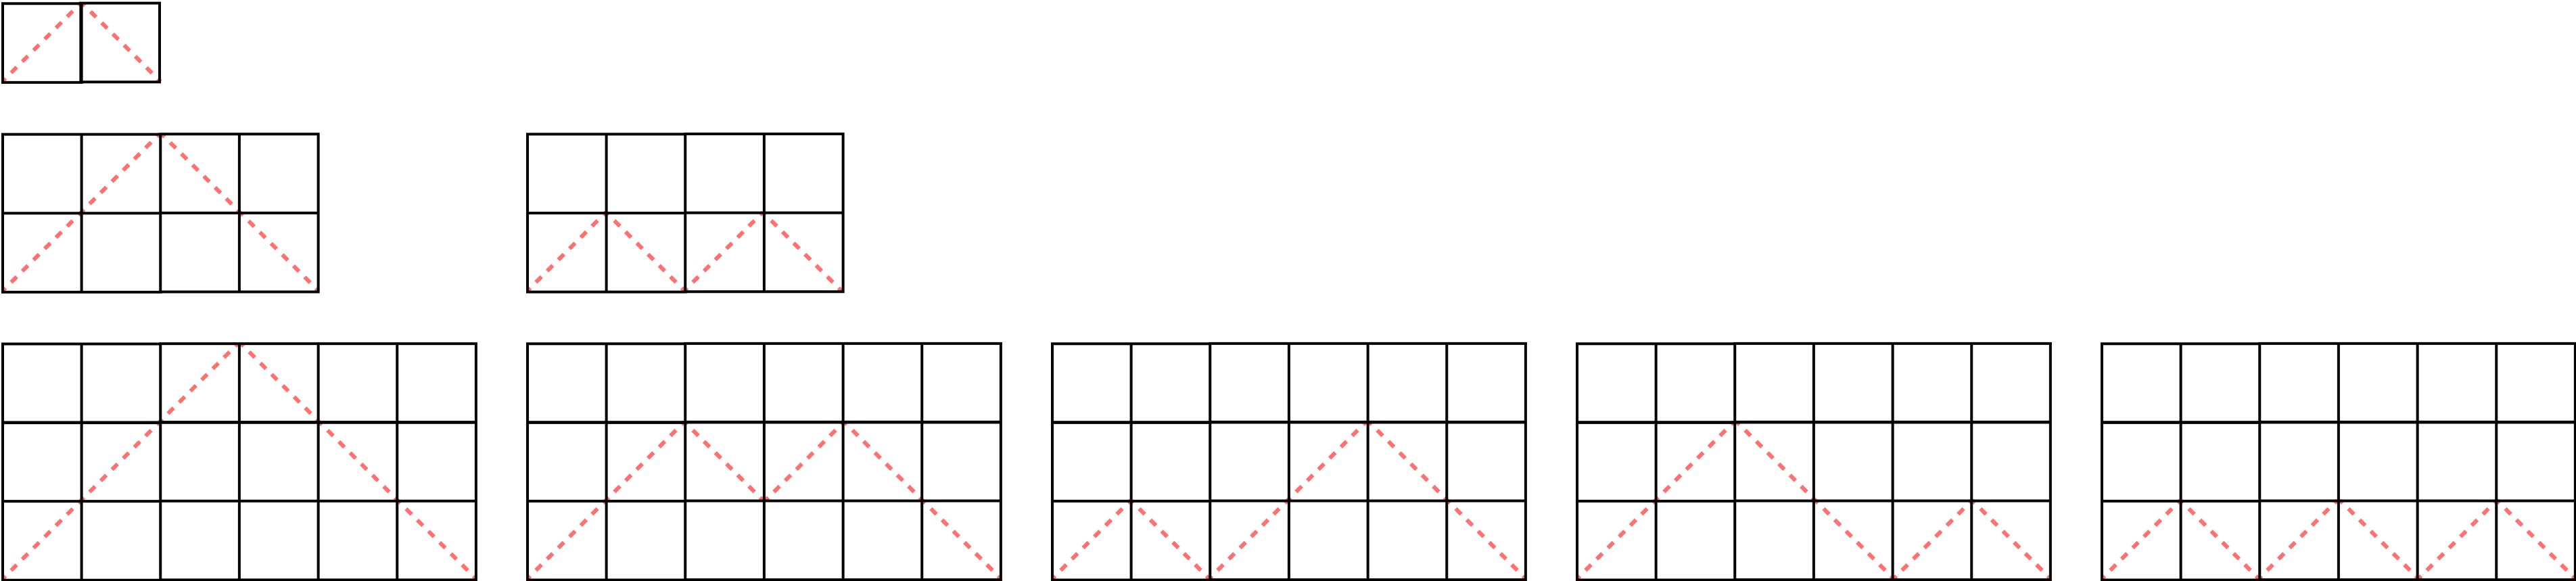
\includegraphics[width=1.2\linewidth]{Images/Figure13.png}
    \caption{All possible Dyck paths from  $(0,0)\to (2n,0)$ for $n=1,2,3$}
    \label{f:3.23}
\end{figure}
Once again, a bijection presents itself when \cref{f:3.21} and \cref{f:3.23} are compared. Namely, the entries in the first row of the $2\times n$ grid correspond to when an up-step in our Dyck path occurs, and the entries in the second row correspond to when a down-step in our Dyck path occurs.     
\end{solution}
\begin{question}
Count the number of ways $a_5(n)$, of joining $n$ non-intersecting chords on a circle marked with $2n$ points.     
\end{question}
\begin{solution}
\begin{figure}[H]
    \centering
    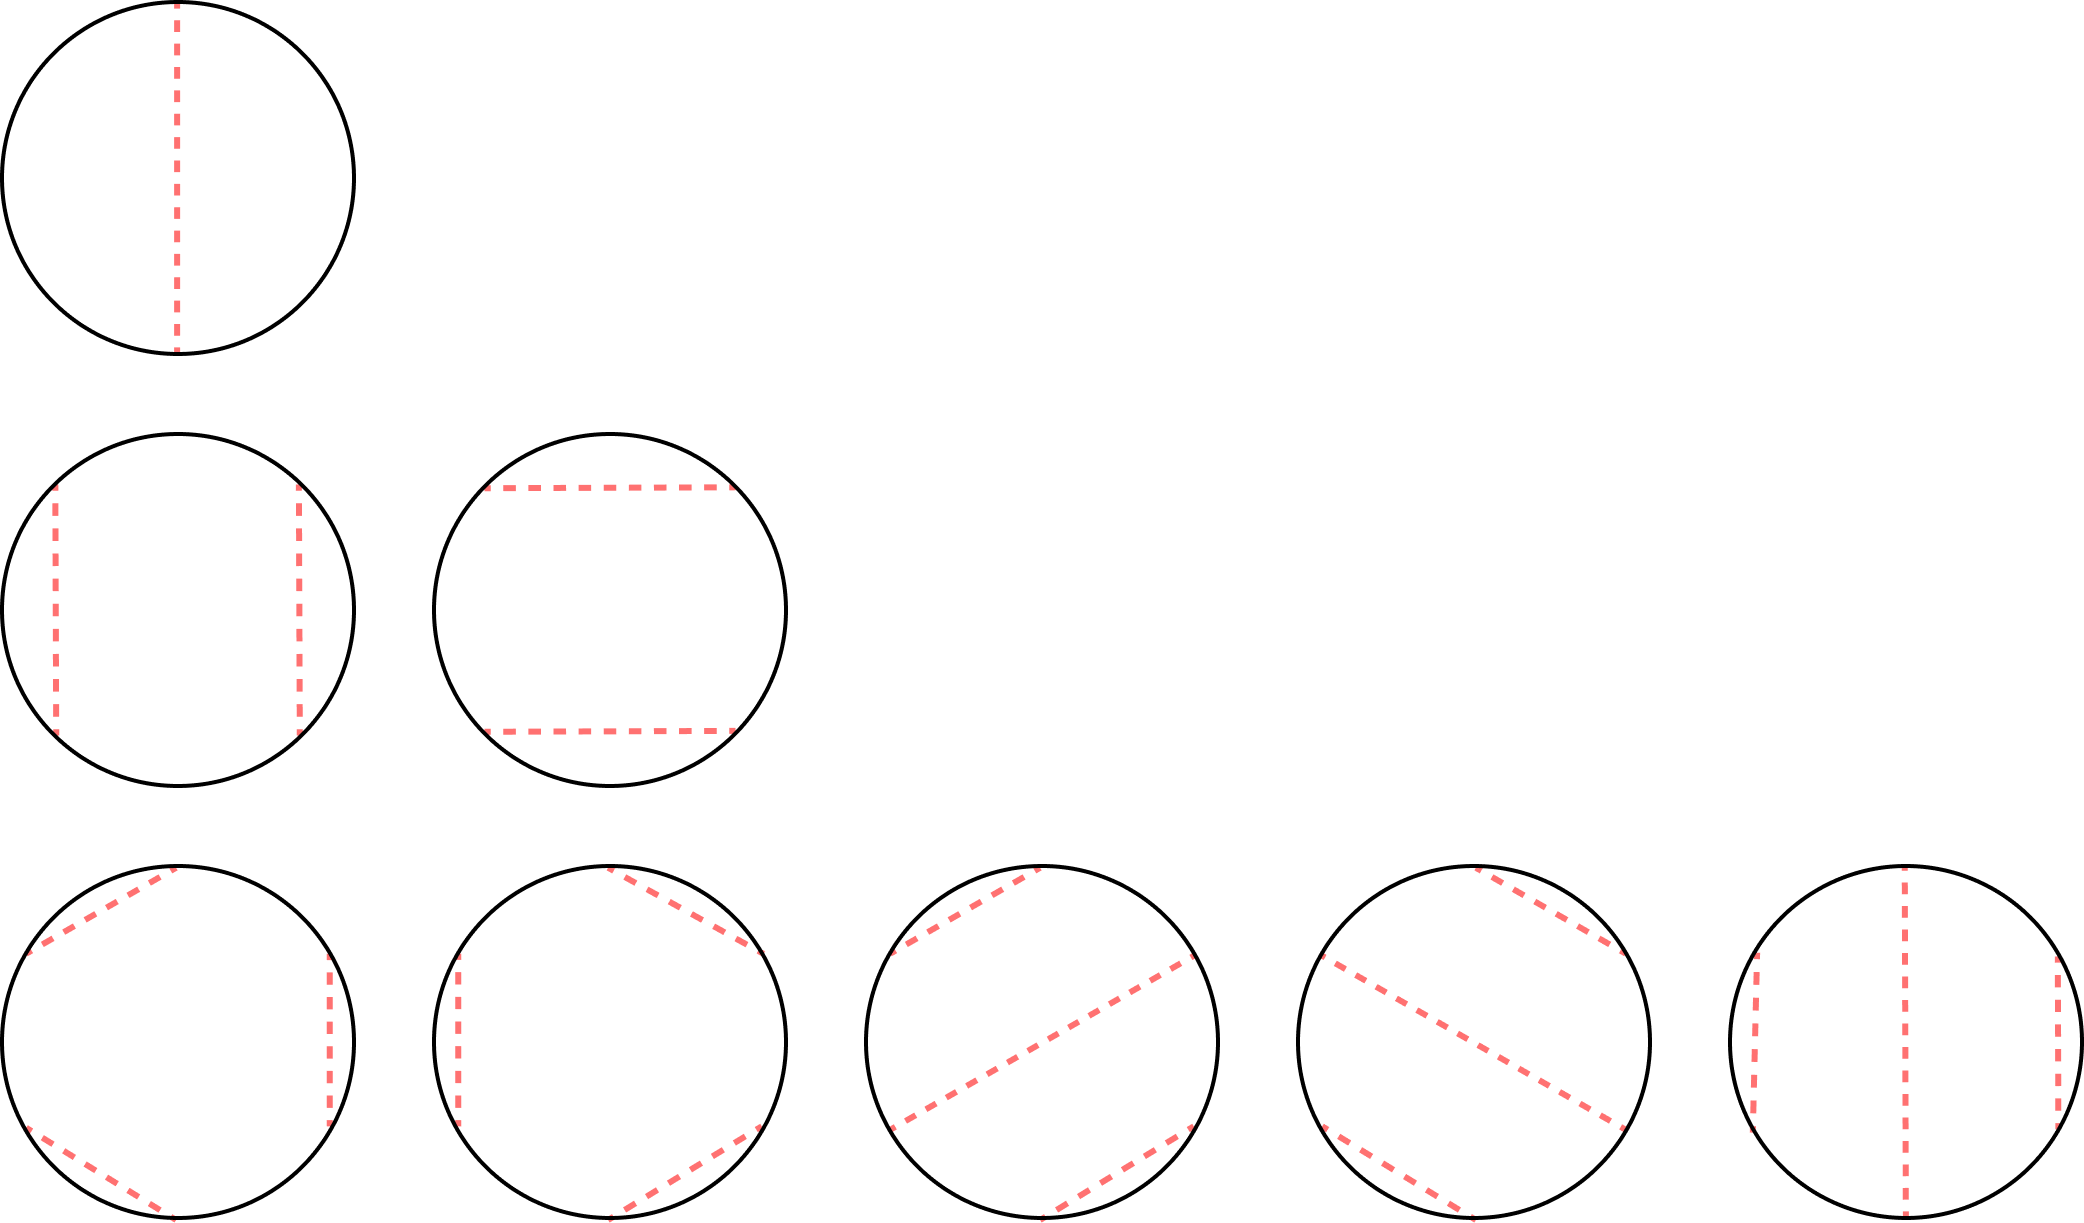
\includegraphics[width=0.8\linewidth]{Images/Figure14.png}
    \caption{All possible such configurations for cases $n=1,2,3$}
    \label{f:3.24}
\end{figure}
Once again, a bijection presents itself when \cref{f:3.22} and \cref{f:3.24} are compared. Namely, if $p_1,\cdots,p_{2n}$ are the marked points on the circle, then we join $p_i$ and $p_j$ if and only if $i$ occurs below $j$ in the arranged grid of numbers. 
\end{solution}
\begin{question}
Count $a_6(n)$, the number of legal sequences of $2n$ parentheses. Where, by a legal sequence of parentheses we mean one in which the parentheses can be properly matched, i.e., each opening parenthesis should be matched to a closing one that lies further to its right. We count these for $n=1,2,3$.
\begin{align*}
    & n=1: \quad \left(\right) \\
    & n=2: \quad \left(\left(\right)\right), \left(\right)\left(\right) \\
    & n=3: \quad \left(\left(\left(\right)\right)\right), \left(\right)\left(\left(\right)\right), \left(\left(\right)\right)\left(\right), \left(\right)\left(\right)\left(\right)
\end{align*}
Once again, notice how corresponding to each grid in \cref{f:3.22} there is a legal sequence of parentheses. Namely, for each entry in the first row, we open a parenthesis, and close it for each entry in the second row.    
\end{question}
\begin{question}
Count $a_7(n)$, the number of non-crossing partitions on the set $[2n]:=\{1,2,3,\cdots,2n\}$. Where by a non-crossing partition on $[2n]$ we refer to an arrangement of $2n$ points on a line, with $n$ non-intersecting arcs joining them.    
\end{question}
\begin{solution}
\begin{figure}[H]
    \centering
    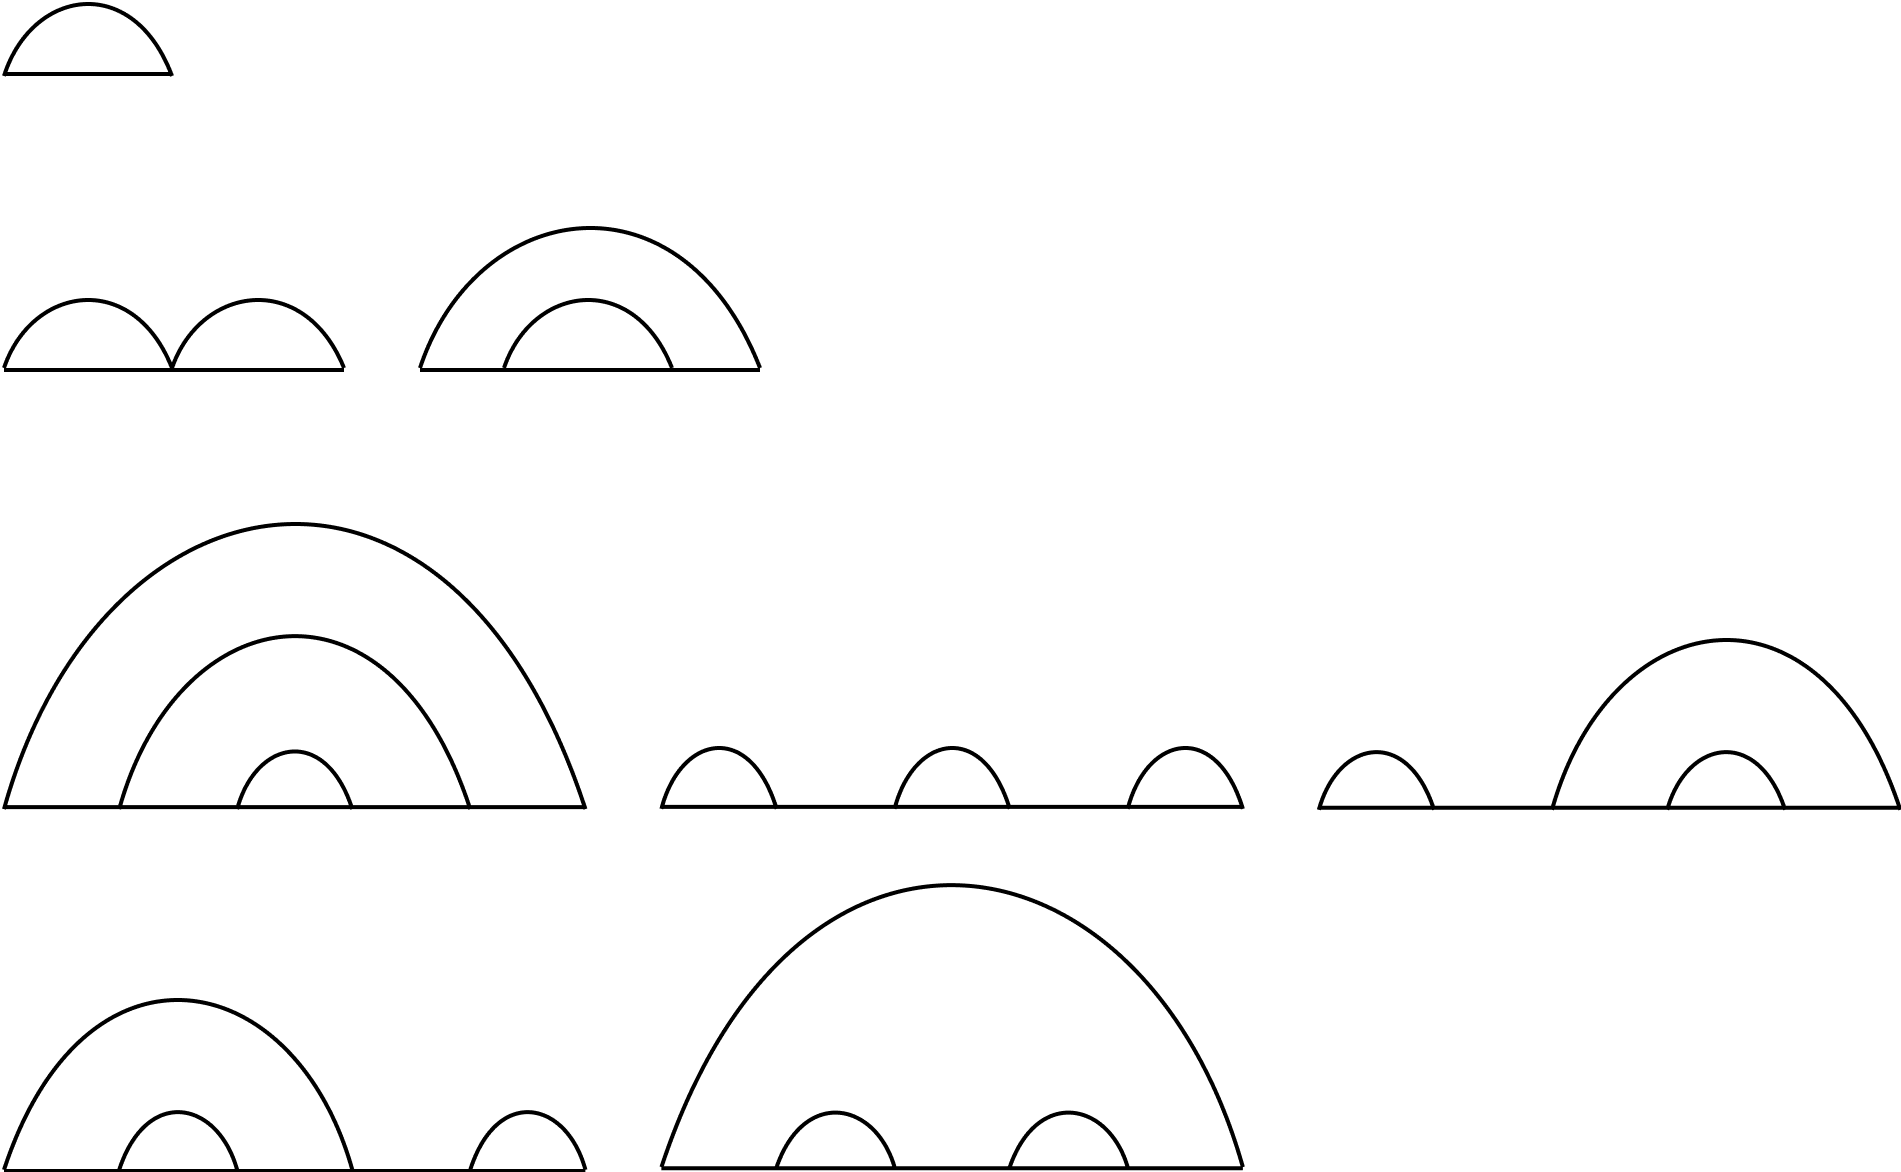
\includegraphics[width=0.8\linewidth]{Images/Figure15.png}
    \caption{All possible non-crossing partitions on $[2n]$ for $n=1,2,3$}
    \label{f:3.25}
\end{figure}
Once again, a bijection presents itself when \cref{f:3.22} and \cref{f:3.25} are compared. Namely, if $p_1,\cdots,p_{2n}$ are the marked points on the line, then we join $p_i$ and $p_j$ if and only if $i$ occurs below $j$ in the arranged grid of numbers. 
\end{solution}
To summarize, by the many bijections we have set up, $C(n):=a_1(n)=a_2(n)=\cdots=a_7(n)$ for all $n\geq 0$. Additionally, we have also seen that $A(n)$ takes values $1,1,2$ and $5$ for when $n=0,1,2$ and $3$ respectively. Motivated readers may check why and how $C(4)=14$, $C(5)=42$, and so on, but this is not how we want to proceed. Consider the following definitions.
\begin{definition}[Triangulation]
A triangulation of a convex polygon with $n+2$ vertices $\mathcal{P}_{n+2}$, is a set of $n-1$ diagonals that do not cross each other in the interior of $\mathcal{P}_{n+2}$. 
\end{definition}
\begin{remark}
For instance, the $3$-gon (triangle) has no triangulations, but the $4$-gon (square/rectangle) has $2$.    
\end{remark}
\begin{definition}[Catalan Numbers]
The sequence $C(n)$ which counts the the number of triangulations of $\mathcal{P}_{n+2}$ is called the sequence of Catalan numbers.
\label{d:catalan}
\end{definition}
\begin{theorem}
For all $n\geq 0$ we have
\[
C(n+1) = \sum_{k=0}^{n}C(k)C(n-k)
\]
\label{t:segner}
\end{theorem}
\begin{figure}[H]
    \centering
    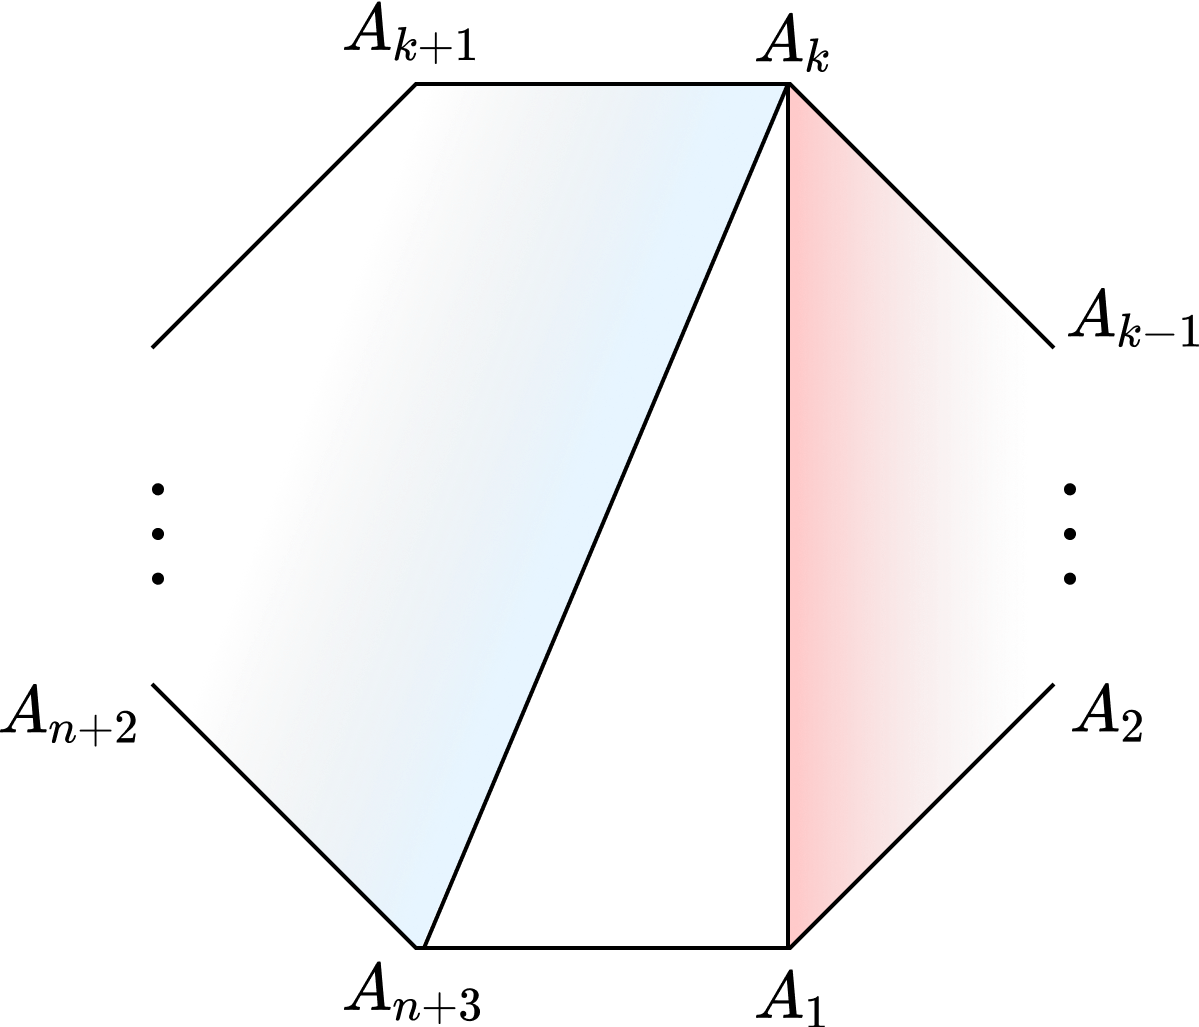
\includegraphics[width=0.45\linewidth]{Images/Figure16.png}
    \caption{}
    \label{f:3.26}
\end{figure}
\begin{proof}
Let $\mathcal{P}_{n+3}$ be an $n+3$ convex polygon with vertices $A_1,\cdots,A_{n+3}$. Next, pick an arbitrary vertex $A_k$ and consider the triangle $\Delta A_1A_{n+3}A_{k}$. See \cref{f:3.26} and notice how this choice splits $\mathcal{P}_{n+3}$ into two convex polygons. One with $k$ vertices (marked red) and the one with $n-k+4$ vertices (marked blue). Since $k$ is allowed to vary from $2$ to $n+2$, by \cref{d:catalan} we have $\sum_{k=2}^{n+2}C(k-2)C(n-k+2)$ ways to triangulate $\mathcal{P}_{n+3}$. Finally, shifting the index of summation by $2$ grants the required result. 
\end{proof}
\begin{claim}
\[
C(n) = \dfrac{1}{n+1}\binom{2n}{n}
\]
\end{claim}
\begin{proof}
Let \[f(x) = \sum_{n=0}^{\infty}C(n)x^n\] be the generating function corresponding to the Catalan numbers. By \cref{t:segner},
\begin{align*}
    f(x)^2 &= C(0)^2 + (C(0)C(1)+C(1)C(0))x + \cdots + (C(0)C(n)\\ &\quad +C(1)C(n-1)+\cdots+C(n)C(0))x^n + \cdots \\
    &= C(1)+C(2)x+\cdots+C(n+1)x^n+\cdots \\
    &= \dfrac{C(x)-C(0)}{x}.
\end{align*}
Solving for $C(x)$ gives \[
C(x) = \dfrac{1\pm \sqrt{1-4x}}{2x}.
\]
Since $C(n)$ is always positive, we discard \[
C(x) = \dfrac{1+ \sqrt{1-4x}}{2x}.
\] and expand $\sqrt{1-4x}$ using \cref{t:2.3rev} to see why 
\[
C(x) = \sum_{n=0}^{\infty}\dfrac{1}{n+1}\binom{2n}{n}x^n.
\]
\end{proof}
\begin{remark}
Catalan numbers come up in a huge class of counting problems. Richard Stanley, in his book, ``Catalan Numbers'' outlines $214$ such problems. That being said, the many bijections we have outlined in this section are not always as easy to find. In such cases, the defining recurrence (\cref{t:segner}) we have obtained is particularly useful. Consider the following example for instance.
\end{remark}
\begin{question}
Count the number of binary trees with $n$ vertices.
\end{question}
\begin{figure}[H]
    \centering
    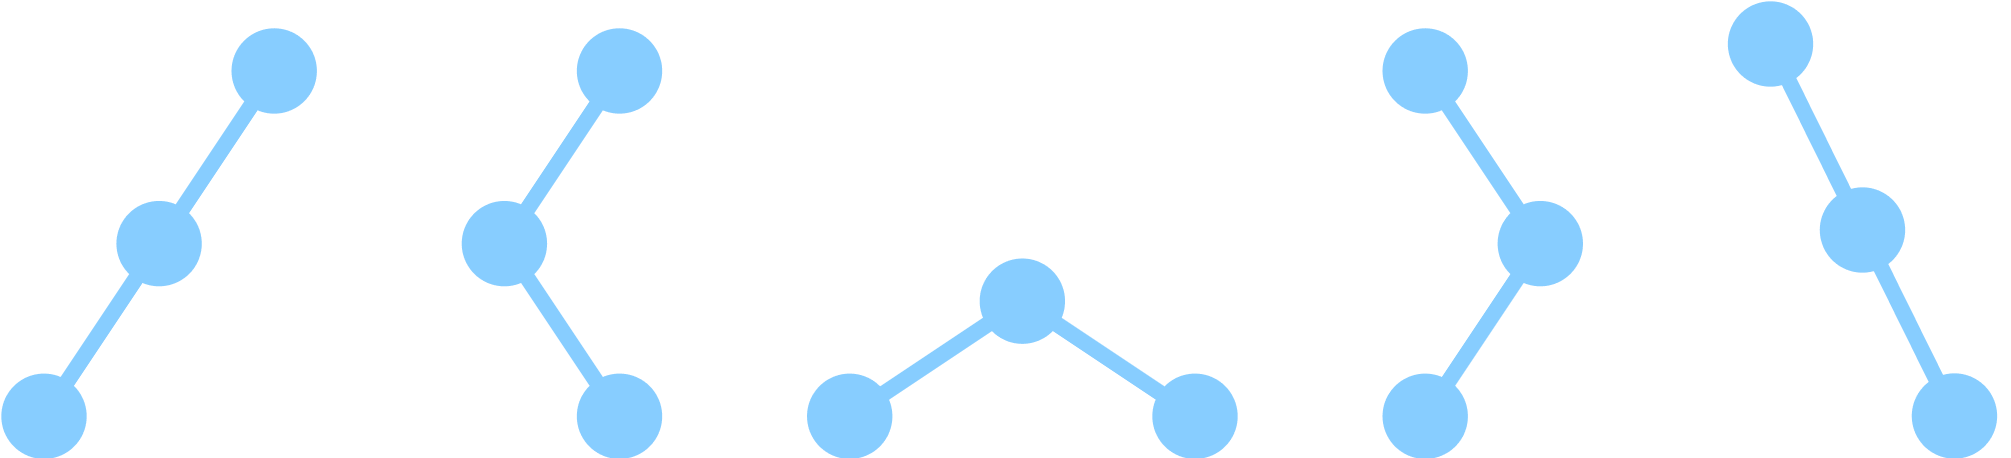
\includegraphics[width=0.7\linewidth]{Images/Figure23.png}
    \caption{The $5$ binary trees on $3$ vertices.}
\end{figure}
\begin{solution}
Let $a_n$ denote the number of binary trees with $n$ vertices, where $n\geq 0$. Since the empty tree is the only binary tree with $0$ vertices, it is clear why $a_0 = 1$. Similarly, it is also clear why $a_1=1$. Consider a binary tree $T$ (say) with $n$ vertices. The root of $T$ has $n-1$ children. For a choice of $0\leq i\leq n-i-1$ let $T$ have $i$ children on the left sub-tree and $n-i-1$ children on the right. By our set-up, there are $a_i$ binary trees with $i$ vertices and $a_{n-i-1}$ binary trees with $n-i-1$ vertices. It follows that there are $a_i a_{n-i-1}$ binary trees with $i$ children on their left subtrees and $n-i-1$ children on their right. Thus, the total number of binary trees with $n$ vertices is given by
\[
a_n = \sum_{i=0}^{n-1}a_ia_{n-i-1}.
\]
Comparing with \cref{t:segner} we get that $a_n$ is counted by the Catalan numbers. 
\end{solution}
We are now interested in stating a recurrence for Catalan numbers which is different from the one we already stated. To this end consider the following theorem and its corollary. 
\begin{theorem}
    Let $T_n$ be the number of triangulations of an $n$-gon, then for $n\geq 4$,
    \[
    (2n-6)T_n = n\sum_{k=3}^{n-1}T_kT_{n-k+2}
    \]
\end{theorem}
\begin{figure}[H]
    \centering
    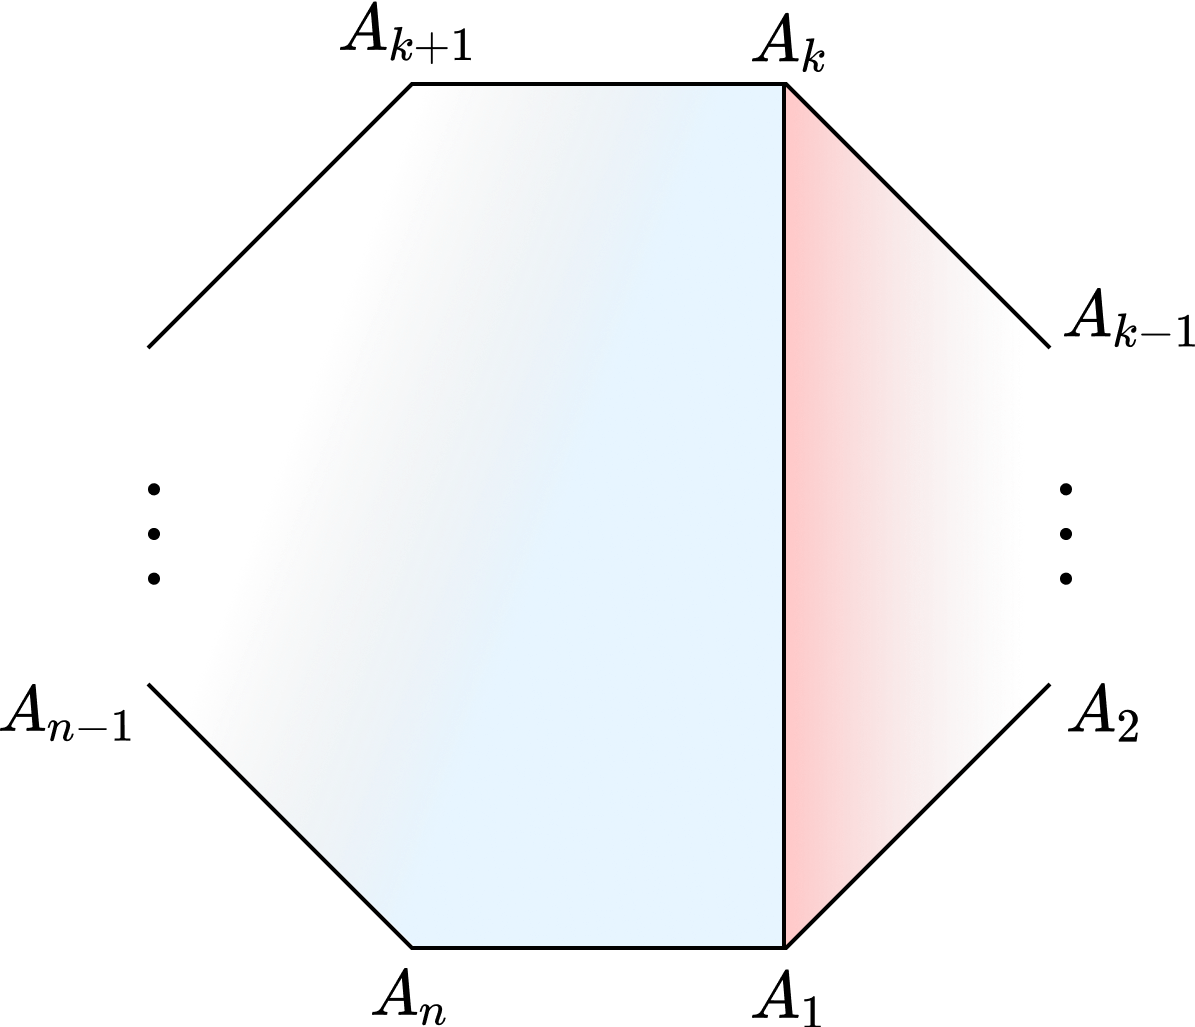
\includegraphics[width=0.45\linewidth]{Images/Figure22.png}
    \caption{}
    \label{f:Segner2f}
\end{figure}
\begin{proof}
Consider an $n$-gon with vertices $A_1,A_2,\ldots,A_n$. Conisder an arbitrary diagonal $\overline{A_1A_k}$ leaving $A_1$, where $2<k<n$. See \cref{f:Segner2f} and notice how this partitions the $n$-gon into the $k$-gon $A_1A_2\ldots A_k$ (marked red) and the $(n-k+2)$-gon $A_1A_kA_{k+1}\ldots A_n$ (marked blue). The $k$-gon can be triangulated in $T_k$ ways and the $(n-k+2)$-gon in $T_{n-k+2}$ ways. It follows that the $n$-gon can be triangulated in a total of $T_kT_{n-k+2}$ ways. Since $k$ is allowed to vary between $3$ and $n-1$, it also follows that the total number of triangulations based at $A_1$ are given by \[
\sum_{k=3}^{n-1}T_kT_{n-k+2}.
\]
Our choice of $A_1$ is not special. Since there $n$ choices of vertices where the triangulation can be based one might think the count is
\[
n\sum_{k=3}^{n-1}T_kT_{n-k+2}.
\]
However, we have overcounted. More specifically, the diagonals $\overline{A_iA_j}$ are counted twice. This gives;
\[
n/2\sum_{k=3}^{n-1}T_kT_{n-k+2}.
\]
Finally, since the $n$-gon has $n-3$ diagonals at every vertex and every triangulation uses $n-3$ diagonals, it follows that
\[
(n-3)T_n = n/2\sum_{k=3}^{n-1}T_kT_{n-k+2}.
\]
as required.
\end{proof}
A corollary follows naturally.
\begin{corollary}
\[
(2n-2)C_n = (n+2)\sum_{k=1}^{n-1}C_kC_{n-k}
\]
\end{corollary}